\section{eo\-Weak\-Elitist\-Replacement$<$ EOT $>$ Class Template Reference}
\label{classeo_weak_elitist_replacement}\index{eoWeakElitistReplacement@{eoWeakElitistReplacement}}
eo\-Weak\-Elitist\-Replacement: a wrapper for other replacement procedures.  


{\tt \#include $<$eo\-Replacement.h$>$}

Inheritance diagram for eo\-Weak\-Elitist\-Replacement$<$ EOT $>$::\begin{figure}[H]
\begin{center}
\leavevmode
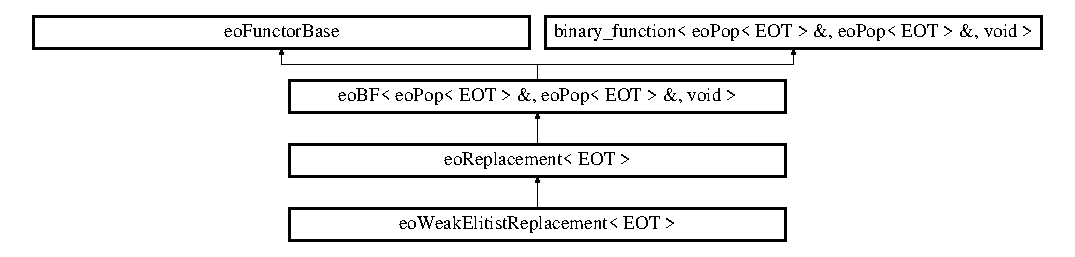
\includegraphics[height=3.01075cm]{classeo_weak_elitist_replacement}
\end{center}
\end{figure}
\subsection*{Public Types}
\begin{CompactItemize}
\item 
typedef EOT::Fitness {\bf Fitness}\label{classeo_weak_elitist_replacement_w0}

\end{CompactItemize}
\subsection*{Public Member Functions}
\begin{CompactItemize}
\item 
{\bf eo\-Weak\-Elitist\-Replacement} ({\bf eo\-Replacement}$<$ {\bf EOT} $>$ \&\_\-replace)\label{classeo_weak_elitist_replacement_a0}

\item 
void {\bf operator()} ({\bf eo\-Pop}$<$ {\bf EOT} $>$ \&\_\-pop, {\bf eo\-Pop}$<$ {\bf EOT} $>$ \&\_\-offspring)\label{classeo_weak_elitist_replacement_a1}

\begin{CompactList}\small\item\em do replacement \item\end{CompactList}\end{CompactItemize}
\subsection*{Private Attributes}
\begin{CompactItemize}
\item 
{\bf eo\-Replacement}$<$ {\bf EOT} $>$ \& {\bf replace}\label{classeo_weak_elitist_replacement_r0}

\end{CompactItemize}


\subsection{Detailed Description}
\subsubsection*{template$<$class EOT$>$ class eo\-Weak\-Elitist\-Replacement$<$ EOT $>$}

eo\-Weak\-Elitist\-Replacement: a wrapper for other replacement procedures. 

Copies in the new pop the best individual from the old pop, AFTER normal replacement, if the best of the new pop is worse than the best of the old pop. Removes the worse individual from the new pop. This could be changed by adding a selector there... 



Definition at line 102 of file eo\-Replacement.h.

The documentation for this class was generated from the following file:\begin{CompactItemize}
\item 
eo\-Replacement.h\end{CompactItemize}
